\documentclass{mcmthesis}
\mcmsetup{CTeX = false, 
        tcn = 2121702, problem = C,   % 修改控制号和选题号
        sheet = true, titleinsheet = true, keywordsinsheet = true,
        titlepage = false, abstract = true}
\usepackage{palatino}
\usepackage{lipsum}
\usepackage{amsmath}  % 此处引入数学公式的包
\usepackage{graphicx} % 用于插入图片
\usepackage{subfigure}
\usepackage{float}
\usepackage{caption2}
 
% 控制页 %%%%%%%%%%%%%%%%%%%%%%%%%%%%%%%%%%%%%%%%%%%%%%%%%%%%%%%%%%%%%%%
% 论文标题
\title{The \LaTeX{} Template for MCM Version \MCMversion}  % 修改标题
\date{\today}
 
\begin{document}
\begin{abstract}
% 摘要部分
% Here is the main abstract part. \\ Go to the next line.
% 关键词
\begin{keywords}  
keyword1; keyword2
\end{keywords}
\end{abstract}
 
% 目录页 %%%%%%%%%%%%%%%%%%%%%%%%%%%%%%%%%%%%%%%%%%%%%%%%%%%%%%%%%%%%%%%%
\maketitle         % 控制序列
\tableofcontents   % 生成目录
\newpage
 
% 基础用法 %%%%%%%%%%%%%%%%%%%%%%%%%%%%%%%%%%%%%%%%%%%%%%%%%%%%%%%%%%%%%%%
 
% 标题 -----------------------------------------
\section{Introduction}
\subsection{Background}
\subsection{Problem restatement}
\section{Assumption and nomenclature}
\section{Model1-Prediction of pest spread over time}
\subsection{Date processing}
The right way of thinking about data processing is the beginning of good modeling. According to the prompt of the question, we first build the database based on “Global ID”, the unique primary key of all text, images and videos, in order to better sort out the relationship between data. The availability and reliability play fundamental role in the establishment of the model. For the purpose of addressing and discussing the prediction of the pest ,we can undoubtedly only keep those sightings that are confirmed as "positive" by USDA staff.

In addition, we had to retrieve biological information related to the spread of hornets from Annex 1, as follows

\begin{itemize}
\item Queen hornets search for new habitats every spring
\item The spread of hornets is less than 30km per year
\item Only the queen bee can survive the winter
\end{itemize}

In order to make preliminary observations on the pattern of hornet propagation in the remaining data, we should classify, sort, sieve and visualize the data in the dataset according to different information dimensions, as follows.

Step1: Mark all 14 hornet occurrence points on Google Earth based on the latitude and longitude of each data entry and label the events.

Step2: All the wasps were marked with different colors according to the year of their appearance, and a line was formed with each year.

Step3: Circle the range they can spread in the next year in proportion to the actual distance

The pictures of each step are as follows:

\begin{figure}[H]
\centering
\subfigure[POSTIVE1]{
    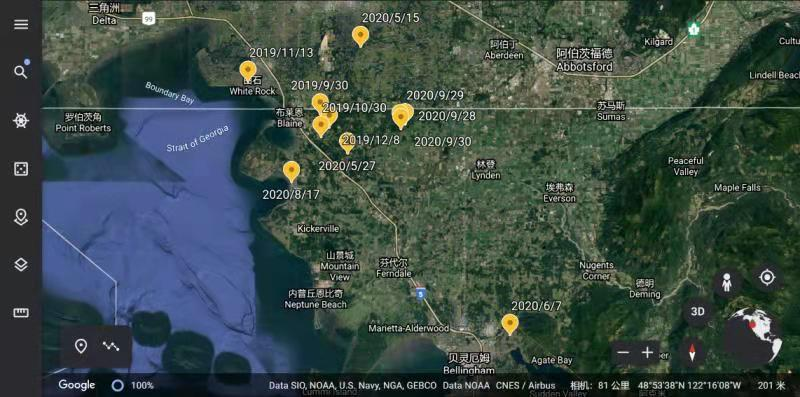
\includegraphics[width=0.45\textwidth]{img/1.png}
}
\subfigure[POSTIVE2]{
    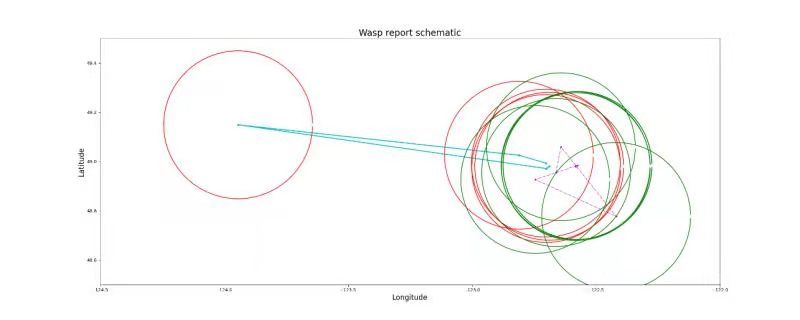
\includegraphics[width=0.45\textwidth]{img/2.png}
}
\caption{POSTIVE}
\label{POSTIVE}
\end{figure}

\subsubsection{Data analysis and modeling ideas}
After processing , data were analyzed and found that:

\begin{enumerate}
    \item the earliest positive event occurred in 2019.
    \item hornets were present on both sides of the river in 2019. 
    \item The closest distance of hornets appearing on both sides of the river in 2019 is 80km.
    \item No definitive hornet sightings on Vancouver Island on the west bank of the Post River in 2019.
    \item Most of the green dots appear in the southeast of the red dots.
    \item The chances are that the second year's hornets will not stay in the same position as the previous year.
\end{enumerate}

Based on the above findings, we can make the following guesses and inferences about the spread of hornet populations:

\begin{enumerate}
    \item We can guess based on the first three analyses that the hornets invaded this area by water transport around 2018-2019.
    \item The spread of hornets is disturbed by certain external factors and is not completely random. After checking the relevant materials, the southwestward migration bias may be influenced by the northwest wind blowing from the Pacific Ocean in spring.
    \item Based on the last two analyses and the biological characteristic that only hornet queens can survive the winter, we believe that the invasion of hornets is more like a migration than a spread.
\end{enumerate}

To further test the above conjecture, we quantified the data as follows:

Step 1 :We find the geometric centroid of the location of the hornet in 2019 2020 respectively (note that Vancouver Island is too far away in 2019 to be counted in the calculation) and calculate their relative displacement \[coordinatesD:(\mu_1,\mu_2)=(9.5,3.7).\]

Step2:  Calculate the standard deviation of the change in the horizontal and vertical coordinates of each point in 2020 with respect to the geometric centroid in 2019.
\[\delta_1=8.40,\delta_2=7.04\]

Step3.   We use equation
\begin{equation}
r=\frac{\sum(X-\Bar{X})(Y-\Bar{Y})}{\sqrt{\sum(X-\Bar{X})^2\sum(Y-\Bar{Y})^2}}
\label{1}
\end{equation}

 to calculate the correlation coefficient matrix between the change in horizontal and vertical coordinates in 2020 compared to 2019.
 
 Since the origin of the wasp invasion is not known, we could not find the location of the wasp in the previous year by the location of its appearance in 2020. However, we consider the invasion of hornets as something near 2019, so here it is useful to approximate the center of all points in 2019 as the point of origin of hornets, and to study and model the probability of hornet spread based on this point for each point distribution in 2020.
    
\subsection{A probabilistic model for the spread of hornets}
Hypothesis:
\begin{enumerate}
    \item Consider the migration of a queen hornet in spring as a mass movement on the coordinate axis
    \item The starting point of the hornet queen of the previous year is the point (0, 0) of the coordinate axis.
    \item A hornet queen moves in a circular coverage area with a radius of 30km at a time.
    \item The distribution of hornet colonies in the movable range approximates some kind of Gaussian distribution.
\end{enumerate}

We assume that the probability of the hornet queen moving from the position (0, 0) in the first year to any point M :$(x, y)$ is PM .Based on the already calculated relative displacement of 2020 compared to the 2019 geometric center point D:$(\mu_1,\mu_2)$ , we consider that the center of the sample distribution of PM should be in(9.5,3.7).
According to the assumption, the distribution of PM obeys the Gaussian distribution with the formula:

\begin{equation}
f(x,y)=(2\pi\delta_1\delta_2\sqrt{1-\rho^2})^{-1} exp[-\frac{1}{2(1-\rho^2)}(\frac{(x-\mu_1)^2}{\delta_1^2}-\frac{2\rho(x-\mu_1)(y-\mu_2)}{\delta_1\delta_2}+\frac{(y-\mu_2)^2}{\delta_2^2})]
\label{2}
\end{equation}
where the parameter $\delta_1=8.40,\delta_2=7.04, \mu_1=9.5,\mu_1=3.7,\rho=|r|=0.688$

The above is the probability distribution of the spread of hornets in a year.

We used python software to plot its probability distribution surface as shown in the figure.

\begin{figure}[H]
    \centering
    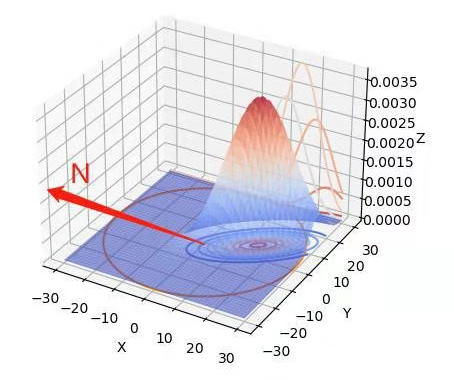
\includegraphics[width=0.8\textwidth]{img/3.png}
    \caption{POSTIVE}
    \label{POSTIVE}
\end{figure}

We found that a portion of the points were distributed beyond the theoretically movable range, and we could not fully accept the model at the 99.74 percent level according to the 3σ principle. Therefore, we can find the sum of the probabilities of all points distributed within the theoretical range by means of definite integration as the accuracy of our model.

The general idea of solving the definite integral in python is to cut all the areas in the ring horizontally and then vertically into as many squares of equal length and width and different heights as possible, take a point in each piece to find the value of the function of the corresponding surface to find the volume of the rectangle, and then add up these small rectangle volumes separately to get the solution of the definite integral.

The solution code is as follows:

\begin{figure}[H]
    \centering
    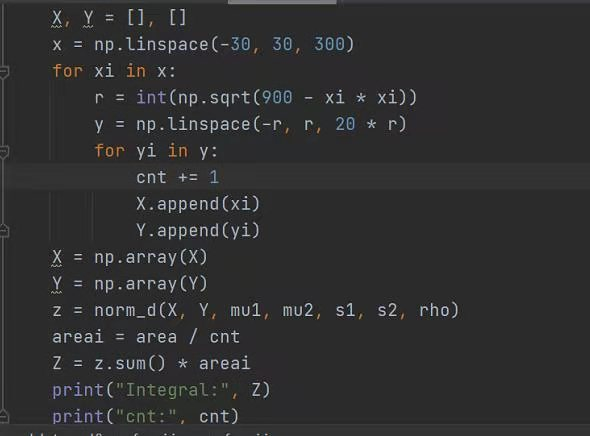
\includegraphics[width=0.6\textwidth]{img/4.png}
    \caption{POSTIVE}
    \label{POSTIVE}
\end{figure}

The calculated accuracy results are:

\begin{figure}[H]
    \centering
    
\includegraphics[width=0.8\textwidth]{img/5.png}
    \caption{POSTIVE}
    \label{POSTIVE}
\end{figure}

\section{Logistic model for predicting the likelihood of a mistaken classification.}

\subsection{Date processing}

To make the data clearer, we sort all the data in the dataset and count what kind of data is available under each “Global ID”.

We found that a sighting usually includes two types of data, text or image, and sometimes a video file. The text file usually includes a description of the hornet by the witness Classified as, and an evaluation of the reported sighting by the researcher, which may be “POSITIVE,NEGATIVE,UNVERIFIED”. The image and video files are all photos of the suspected wasps provided by the witnesses. In addition, there is information about the time and location of the reported sighting and the time of the laboratory's conclusion.

\begin{figure}[h]
    \centering
    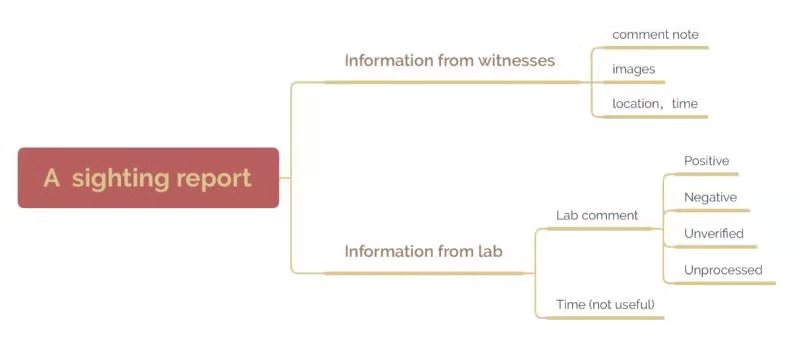
\includegraphics[width=0.8\textwidth]{img/6.png}
    \caption{POSTIVE}
    \label{POSTIVE}
\end{figure}

\subsection{Analysis of model}

This is a typical classification prediction model for predicting the wrongness of any sighting event. We need to analyze the statistics of the different dimensions of information carried by the sample of sighting reports to analyze how they determine the evaluation of the lab. Some of the factors that can be taken into account that can have an impact on the results of the laboratory evaluation are the following:

\begin{enumerate}
    \item Location of the incident report
    \item Date of detection
    \item Adequacy of the report's basis for appraisal by appraisers (with or without pictures)
    \item Is there ambiguity in the written narrative
    \item Is the species in the picture similar enough to the hornet
\end{enumerate}

Hornets have not invaded this area until 2019, so sightings from these years should be removed, and we should exclude "Unverified" events that are of little significance for evaluating model oversight. According to the model of hornet dispersal, it is known that there is a limit to the number of locations a hornet can reach in a given period of time, so we will give a more negative evaluation to events that are outside the possible range. A lower rating may likewise be given in the reporter's own description of the sighting if there is uncertainty in the language. In the absence of visual materials such as pictures, it is often difficult for staff to judge whether it is indeed a hornet, so again we can give a lower rating to this type of report. Finally, image recognition technology is applied to compare the insects in the pictures provided by the sighting with real wasps, and if the similarity is low, a lower score can also be given

The above analysis is at the speculative level, and then we will first quantify these factors and built the model.

\subsection{Model building}

\subsubsection{clean and classify the dataset}
Excluding sightings prior to 2019,Remove all "Unverified" events. The remaining events as sample events are divided into two categories according to 2019 and 2020 . to facilitate the next use.

\begin{figure}[H]
\centering
\subfigure[POSTIVE1]{
    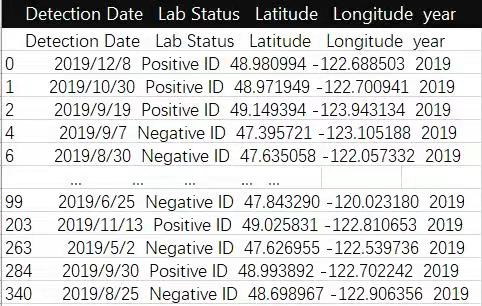
\includegraphics[width=0.42\textwidth]{img/7.png}
}
\subfigure[POSTIVE2]{
    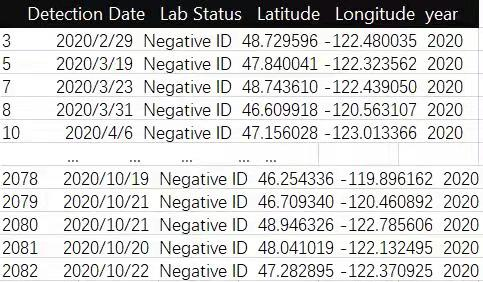
\includegraphics[width=0.45\textwidth]{img/8.png}
}
\caption{POSTIVE}
\label{POSTIVE}
\end{figure}

\subsubsection{Probability based on propagation model}

Based on the hornet dispersal model developed in the first question, we denote the probability of the possible presence of hornets at the place of occurrence at the reporting time as x1 and $x_2=x_1^2$

\subsubsection{ Plain Bayesian classifier model}
We have to obtain useful information from the Notes of the informants in order to assist us in predicting errors. The basic idea is to first count the number of keywords in the dataset and then divide it by the total number of strengths in the dataset to obtain the probability of that value. Based on the obtained probability value we can then use conditional probabilities for classification.

From Bayesian quasi-measures we can obtain:
$$p(c_i|x,y)=\frac{p(x,y|c_i)p(c_i)}{p(x,y)}$$
From this we define the Bayesian classification quasi-measure:
\begin{itemize}
    \item If $p(c_1|x,y) > p(c_2|x,y)$, then belongs to the category $c_1$
    \item If $p(c_1|x,y) < p(c_2|x,y)$, then belongs to the category $c_2$
\end{itemize}

If we use Bayesian quasi-measures, we can calculate the unknown probability values from the known three probability values, i.e., the probability of which comment we are interested in for a particular keyword.
Using this as a basis to start using the plain Bayesian classifier (assuming that the keywords are independent of each other and that the features of the keywords are equally important) 

step1:construct a word vector from the text

step2: incorporate the useful words that appear in Notes into the word vector, while excluding pronouns, predicates, and other words that are not useful for prediction in the utterance.

Step3:build a vocabulary list belonging to the model. 

Once the glossary is obtained, the number of occurrences of the words in the glossary in Notes is counted and sorted. Then we use the training algorithm to calculate the probability from the word vector:

\begin{equation}
p(c_i|\omega)=\frac{p(\omega|c_i)p(c_i)}{p(\omega)}
\label{4}
\end{equation}

where $\omega$ is the word vector

Calculate the probability $p(c_i)$ by dividing the number of Notes in category i(positive、negative、unprocess) by the total number of Notes

Then calculate $p(\omega|c_i)$ using the plain Bayesian assumption Since each word in the word vector is assumed to be independent, the above probabilities can be written:

\begin{equation}
p(x_1|c_i)p(x_2|c_i)p(x_3|c_i)···p(x_n|c_i)
\label{5}
\end{equation}

The calculation process is greatly simplified.

In order to solve the problem of overflow (overflow due to too small multiplication of probabilities), we use the natural logarithm of the product

\begin{equation}
\ln{a*b}=\ln{a}+\ln{b}
\label{6}
\end{equation}

A plain Bayesian classifier has now been implemented, and the classifier successfully extracts the keywords in Notes in Positive ID as well as in Notes in Negative ID and the occurrence of the word with that reported information
is the probability of the corresponding category.

From this, we can give the corresponding ratings as feature values by calculating the keywords in the reported information Notes for further machine learning. The general flow chart is shown below .

\begin{figure}[h]
    \centering
    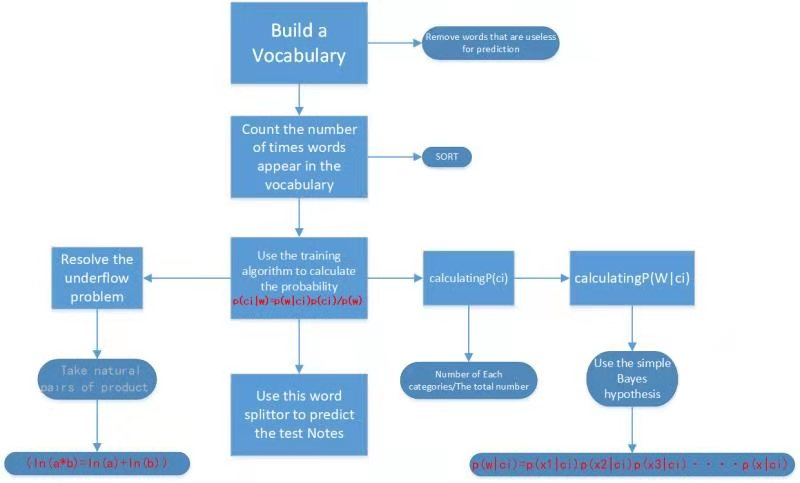
\includegraphics[width=0.8\textwidth]{img/9.png}
    \caption{POSTIVE}
    \label{POSTIVE}
\end{figure}

The following figure shows the results of some higher frequency words in "Positive Note" and "Negative Note" by using Bayesian classifier. These probability indicates the conditional probability that it is” POSITIVE” or” NEGATIVE” after the occurrence of the term. We only need to know the difference obtained by subtracting the NEGATIVE probability from the POSITIVE probability of each word to quantify the contribution of this word to determining whether the report it is in can be predicted accurately.

\begin{figure}[h]
    \centering
    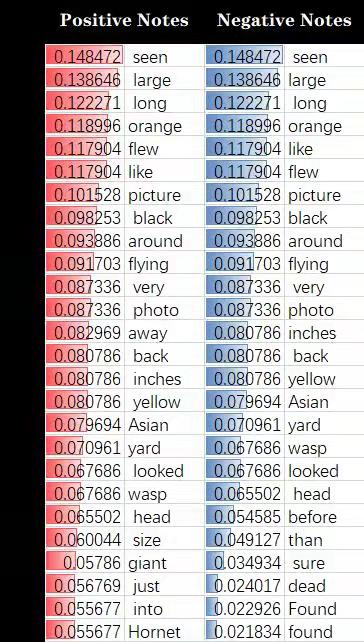
\includegraphics[width=0.8\textwidth]{img/10.png}
    \caption{POSTIVE}
    \label{POSTIVE}
\end{figure}

To describe the effect of Note on the prediction results, we set it as the variable $x_3$. Conditional probability $P(c_i|w)$ for all terms in each reported Note can be accumulated and be regarded as eigenvalue of $x_3$.

\subsubsection{Image recognition model}

We will give importance to reports carrying images or videos in our prediction model, and for this reason, we use the presence or absence of images or videos as a variable x4’.
The eigenvalues of x4 are shown below.


\begin{equation}
    x_4^{'}=\left\{
    \begin{aligned}
        1 &&{,yes} \\
        0 &&{,no}
    \end{aligned}
    \right.
    \label{6}
\end{equation}

If $x_4^{'}=1$ , We will perform image recognition on this image to determine its similarity to the hornet image in "POSITIVE". Then we regard the value of similarity as a significant factor $x_5$ that impressing the judge of prediction model. So the value of $x_5$ is between (0,1). Since $x_5$  is the variable that can only describe the samples carrying the image, while $x_4^{'}$ can describe all samples, we use the variable $x_4$  obtained by multiplying $x_4^{'}$ with $x_5$  as the final variable describing the effect of image factors on the prediction results. 
As for the method of image recognition, the team members, after reviewing the information, chose a machine learning related algorithm.Our team used the existing **Inception model** from **Tensorflow**, divided more than 4000 photos into training and testing sets, and trained and tested their own image recognition AI based on the **Inception model** using **Migration Learning**.

1 .Migration Learning

Transfer Learning attempts to use the parameters of an already trained model to help train a new model on a new data set. When several training tasks and data have some degree of correlation, using transfer learning can speed up the learning of a new model without spending a lot of time and samples to train it from scratch. Our task is an image recognition task, which has a large correlation with Google's trained Inception model, and our samples are small, so migration learning based on the Inception model is a good choice.

2. Inception model

The Inception model is a convolutional neural network model for image classification. It is a multi-layer convolutional neural network with an extremely complex structure. The model can recognize more than 1000 items, but not including the anime characters we want. ram connected to 8 NVIDIA Tesla K40 GPUs). If you want to try to train a neural network of this magnitude from scratch on your PC, you may need several weeks to complete the training, with a high probability of run out of GPU memory or run out of CPU memory leading to training failure. Here we will try to train the last layer of the entire neural network, the decision/classification layer, using retrain.py provided by Tensorflow, while the penultimate layer is called Bottlenecks. We will use the valid data generated by Bottlenecks to feed the final decision layer/classification layer to make the final classification prediction.

The following is the similarity between "Unprocessed" and some "Unverified" hornet images by applying the trained image recognition model.

\subsubsection{Multinomial logistic regression model}

Multinomial logistic regression model is adopted to further assist the Error Likelihood Prediction by composing all factors and unifying them between (0,1). In fact, The prediction error likelihood model has only two possibilities of judgment (wrong, correct). Therefore, the mistaken likelihood of predicting reported hornet sightings is subject to binomial distribution, and logistic model is just suitable for empirical analysis of such kind of data. Multivariate logistic regression can determine the role and intensity of the explanatory variable Xn in predicting the probability of occurrence of strain Y. Suppose that X is the response variable and P is the response probability of the model, and the corresponding regression model is as follows:

\begin{equation}
    \ln{\frac{p_1}{1-p_1}}=\alpha+\sum_{k=1}^k \beta_k\chi_k_i
    \label{6}
\end{equation}

$p_1=p(y_i=1|x_1_i,x_2_i,····,x_k_i)$ is the possibility that case i happens in case the values of $x_1_i,x_2_i,····,x_k_i$ are given. Also $p_1$ is a binomial distribution parameter, and it is the probability that a hornets sighting reported incident predicted to be wrong. $x_k_i$ represents a series of independent variables. $\beta$ is the corresponding estimation coefficient, and α is the intercept, which reflects the random effect at the product level.

The probability of an event happening is a non-linear function composed of the explanatory variable Xi. Here is the expression: 

\begin{equation}
    p=\frac{1}{1+exp[-(\alpha+\beta_1*X_1+\cdot\cdot\cdot+\beta_n*X_n)]}
    \label{6}
\end{equation}

The four variables in the model built in this problem are Propagation Theory Probability and his square, conditional probability of vocabulary, presence or absence of pictures, and similarity of picture recognition, $x_1,x_2,x_3,x_4$ respectively. The eigenvalues of each of these variables xi have been discussed separately above. So our logistic regression equation should be:

\begin{equation}
    p=\frac{1}{1+exp[-(\alpha+\beta_1*X_1+\beta_2*X_2+\beta_3*X_3+\beta_4*X_4)]}
    \label{6}
\end{equation}

We tend to use machine learning to solve the logistic regression equation for the coefficients $\beta_i$: The main principle of the algorithm is the gradient ascent method to find the maximum value of sigmoid function so that $\beta_i$ can be defined.

To implement a logistic regression classifier, we can multiply each characteristic by a regression coefficient, add all the results, and substitute this sum into the Sigmoid function, which in turn yields a range between 0 and 1value. Any data greater than 0.5 is considered positive, while anything less than 0.5 is considered Negative. Therefore, logistic regression can also be considered as a probability estimation.

After determining the functional form of the classifier, we use the random machine gradient ascent algorithm to obtain the best regression coefficients, while avoiding excessive computational complexity, and at the same time perform incremental updates to the classifier as new samples arrive (i.e., online learning algorithm). The difference from the gradient ascent implementation is that the alpha is adjusted for each training and random samples are selected to update the regression coefficients. It is the difference here that makes the stochastic gradient ascent algorithm converges faster and better for the regression coefficients.

Finally, we obtained the coefficients of the four variables by machine learning:

\begin{figure}[H]
    \centering
    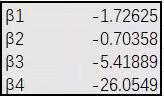
\includegraphics[width=0.3\textwidth]{img/11.png}
    \caption{POSTIVE}
    \label{POSTIVE}
\end{figure}

Therefore:

\begin{equation}
    p=\frac{1}{1+exp{-[(-1.72625)*X_1+(-0.7035)8*X_2+(-5.41889)*X_3+(-26.0549)*X_4]}}
    \label{6}
\end{equation}

The logistic regression model for prediction error is thus derived. The following is the general flow chart for building the model.

Since the response function does not have a constant term $\alpha$, it is possible to derive a threshold value of 0.5 for this prediction model, i.e., when $p > 0.5$ then the prediction is the wrong event, and when $p < 0.5$ then the prediction may be the correct event or an uncertain event.

\begin{figure}[H]
    \centering
    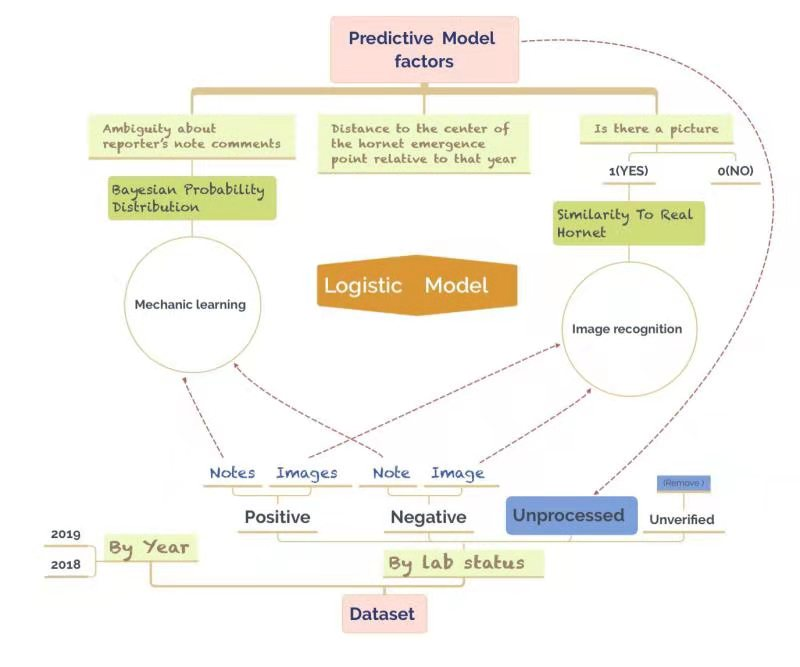
\includegraphics[width=0.8\textwidth]{img/12.png}
    \caption{POSTIVE}
    \label{POSTIVE}
\end{figure}

\subsection{Determine the correct event and its priority based on the error prediction model}

% 行内公式
This is an inline formula. $a = \sqrt{b + c}$.
% 行间公式, 带编号
\begin{equation}
E = mc^2
\end{equation}
\begin{equation}
F = ma
\end{equation}
% 定理
\begin{Theorem} \label{thm:latex}
\LaTeX
\end{Theorem}
% 引理
\begin{Lemma} \label{thm:tex}
\TeX .
\end{Lemma}
% 证明
\begin{proof}
The proof of theorem.
\end{proof}
 
 
% 表格 -------------------------------------------------------
\subsection{Table}
 
\subsubsection{Table-1}
\begin{tabular}{|l|c|r|}
 \hline
OS & Release & Editor\\
 \hline
Windows & MikTeX & TexMakerX \\
 \hline
Unix/Linux & teTeX & Kile \\
 \hline
Mac OS & MacTeX & TeXShop \\
 \hline
General & TeX Live & TeXworks \\
 \hline
\end{tabular}
 
\subsubsection{Table-2}
\begin{tabular}{|r r|}
% r代表row, 使用 | 来划分,如果 r | r中间的|去掉,那么列之间元素无直线划分
\hline
1234 & 5678 \\ \hline
1 &  2 \\ \hline
3 & 4 \\ \hline
\end{tabular}
\subsubsection{Table-3}
\begin{tabular}{ll}
\hline
symbols&definitions\\
\hline
$v_i$& velocity of ball before collision\\
$v_f$& velocity of ball after collision\\
$V_f$& velocity of bat after collision\\
$S$ & the shear modulus the bat\\
$Y$ & Young’s modulus of the bat\\
\hline
\end{tabular}
% 文献引用 %%%%%%%%%%%%%%%%%%%%%%%%%%%%%%%%%%%%%%%%%%%%%%%%%%%
\subsection{Cite}
Here is a example to cite the referenced article\cite{konishi:1999ab}. \\
Another article\cite{refName}.
\section{Analysis of the Problem}
\[
  \begin{pmatrix}{*{20}c}
  {a_{11} } & {a_{12} } & {a_{13} }  \\
  {a_{21} } & {a_{22} } & {a_{23} }  \\
  {a_{31} } & {a_{32} } & {a_{33} }  \\
  \end{pmatrix}
  = \frac{{Opposite}}{{Hypotenuse}}\cos ^{ - 1} \theta \arcsin \theta
\]
\lipsum[9]
\[
  p_{j}=\begin{cases} 0,&\text{if $j$ is odd}\\
  r!\,(-1)^{j/2},&\text{if $j$ is even}
  \end{cases}
\]
\lipsum[10]
\[
  \arcsin \theta  =
  \mathop{{\int\!\!\!\!\!\int\!\!\!\!\!\int}\mkern-31.2mu
  \bigodot}\limits_\varphi
  {\mathop {\lim }\limits_{x \to \infty } \frac{{n!}}{{r!\left( {n - r}
  \right)!}}} \eqno (1)
\]
\section{Calculating and Simplifying the Model  }
\lipsum[11]
\section{The Model Results}
\lipsum[6]
\section{Validating the Model}
\lipsum[9]
\section{Conclusions}
\lipsum[6]
\section{A Summary}
\lipsum[6]
\section{Evaluate of the Mode}
\lipsum[7]
\section{Strengths and weaknesses}
\lipsum[12]
\subsection{Strengths}
\begin{itemize}
\item \textbf{Applies widely}\\
This  system can be used for many types of airplanes, and it also
solves the interference during  the procedure of the boarding
airplane,as described above we can get to the  optimization
boarding time.We also know that all the service is automate.
\end{itemize}
\subsection{Weakness}
\begin{itemize}
\item \textbf{Improve the quality of the airport service}\\
Balancing the cost of the cost and the benefit, it will bring in
more convenient  for airport and passengers.It also saves many
human resources for the airline. 
\end{itemize}
% 引用文献 %%%%%%%%%%%%%%%%%%%%%%%%%%%%%%%%%%%%%%%%%%%%%%%%%%%%%%%
\newpage
\bibliography{article}      % 指定article 代表同目录下的article.bib文件 
\bibliographystyle{ieeetr}  % 定义文献引用的格式
% 附录 %%%%%%%%%%%%%%%%%%%%%%%%%%%%%%%%%%%%%%%%%%%%%%%%%%%%%%%%%
\begin{appendices}
\section{First appendix}
\lipsum[13]
Here are simulation programmes we used in our model as follow.\\
\end{appendices}
\end{document}